\documentclass{beamer}
\usetheme[progressbar=foot, numbering=counter, block=fill]{metropolis}

\AtBeginSection[]
{
  \begin{frame}<beamer>
    \frametitle{Table of Contents}
    \tableofcontents[currentsection]
  \end{frame}
}

\title{Self-paced, assessment based learning (SPABL) in the mathematics classroom}
\date{February 20, 2018}
\author{Jenny Lee}
\institute{Harvey Mudd College\\Advisor: Dagan Karp}
\begin{document}
\maketitle
\section{Introduction}
\subsection{Motivation \& Status Quo}
\begin{frame}{Motivation}
  \begin{center}
    \textit{``Individual differences'' in learners is a fact that can be demonstrated in many ways. That our students {\only<2> {\color{blue}}{vary in many ways}} can never be forgotten ... Our basic task in education is to find strategies which will take individual differences into consideration but which will do so in such a way as to {\only<3> {\color{blue}} promote the fullest development of the individual}.}
  \end{center}
  \hfill- Benjamin Bloom
\end{frame}
\begin{frame}{Status quo - Lecture based}\pause
  \begin{itemize}
    \item Faculty to student ratio $\approx 1:20$ \pause
    \item Generalized instruction, individualized assessment\pause
    \item Common end goal
  \end{itemize}
\end{frame}
\begin{frame}{Status quo - Lecture based}
  \centering
    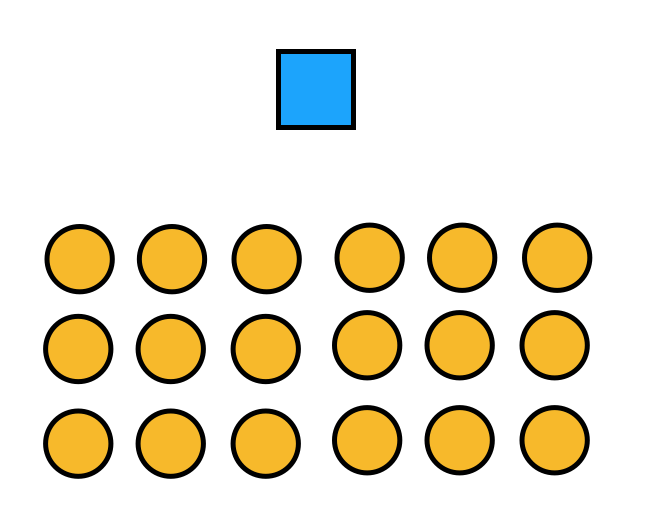
\includegraphics[scale=0.5]{lecturestyle1}
\end{frame}
\begin{frame}{Status quo - Lecture based}
  \centering
    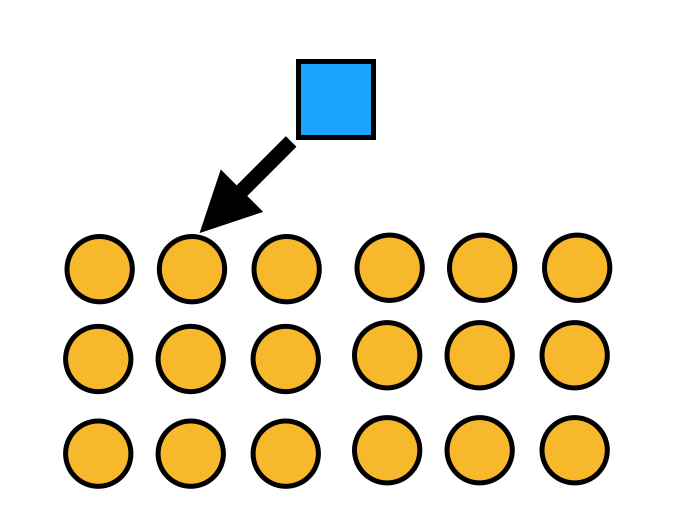
\includegraphics[scale=0.5]{lecturestyle3}
\end{frame}
\begin{frame}{Status quo - Lecture based}
  \centering
    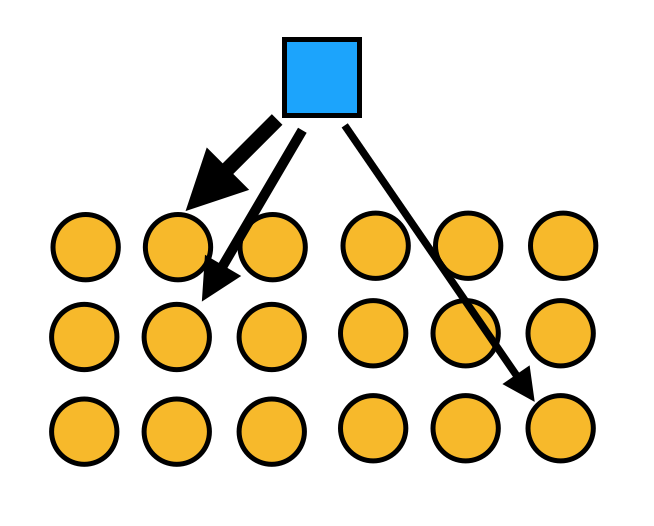
\includegraphics[scale=0.5]{lecturestyle2}\\
    \pause No arrow backwards.
\end{frame}
\section{Mastery learning}
\subsection{Overview}
\begin{frame}{Mastery Learning - overview}
  \begin{itemize}
    \item Developed in 1968 by Benjamin Bloom\pause
    \item Focus on the `mastery' of the subject\pause
    \item Shifting the distribution of achievement upwards\pause
    \item ``Feedback, correction, enrichment''\pause
    \item Repeated assessment, use of TA's
  \end{itemize}
\end{frame}
\begin{frame}{Mastery learning}
  \begin{figure}
    \centering
      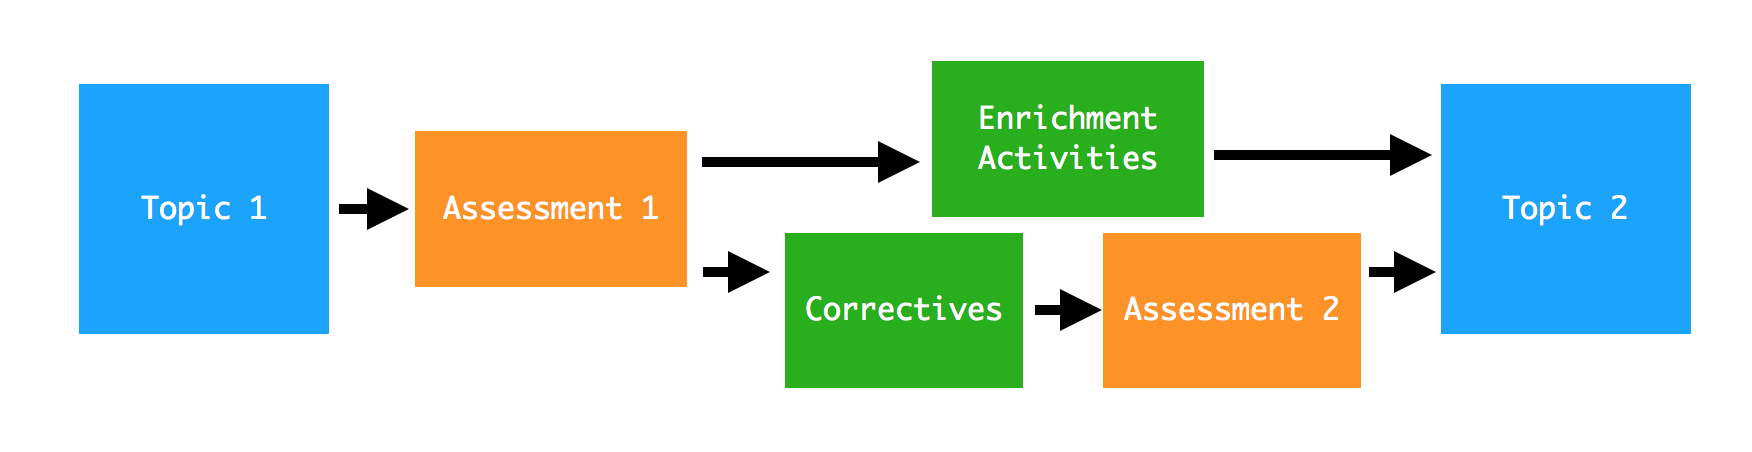
\includegraphics[scale=0.35]{mlflow}
      \caption{Flow chart of typical mastery learning process.}
  \end{figure}
\end{frame}
\subsection{Success in the classroom}
\begin{frame}{Mastery learning - success in the classroom}\pause
  \begin{itemize}
    \item Closing achievement gaps\pause
    \item Self-efficacy (feeling of being capable of independent success)\pause
    \item Enhanced student-teacher relationships
  \end{itemize}
\end{frame}
\subsection{Problems and challenges}
\begin{frame}{Mastery learning - problems and challenges}\pause
  \begin{itemize}
    \item Time-constraints\pause
    \item Demand for more resources\pause
    \item Necessary cuts made to curriculum\pause
    \item Less focus on deeper processing of information or applications
  \end{itemize}
\end{frame}
\section{Self-Paced Assessment Based Learning (SPABL)}
\subsection{Direction}
\begin{frame}{Direction - Modified mastery learning in mathematics}
\begin{itemize}
  \item Keeping the pros of ML, reducing cons\pause
  \item Considerations:\pause
  \begin{itemize}
    \item subject, type of class, size of class
    \item existence of an honor code, TA's, other resources
    \item amount of instructor effort
    \item assessment
  \end{itemize}
\end{itemize}
\end{frame}
\begin{frame}{SPABL - Implementation}
  \begin{itemize}
    \item subject, type of class, size of class {\only<4-> {\color{red} $\to$ introductory math (core math), 20-25 students}}
    \item existence of an honor code, TA's, other resources {\only<5-> {\color{red} $\to$ implementation of supervised or unsupervised numerous small, mandatory assessments for each ``big'' topic}}
    \item amount of instructor effort {\only<6-> {\color{red} $\to$ multiple assessments with multiple tries on each topic}}
    \item accurate assessment of students' understanding {\only<7-> {\color{red} $\to$ ?}}
  \end{itemize}
\end{frame}
\section{Experimentation}
\begin{frame}{Math 40 Experiment}\pause
  \begin{itemize}
    \item Simple implementation of SPABL, A/B testing under same professor with the same material
    \item Students in section A - regular midterm/exam
    \item Students in section B - multiple take-home quizzes with multiple retries without penalty
  \end{itemize}
\end{frame}
\begin{frame}{Math 40 Experiment - current status}\pause
  \begin{itemize}
    \item Perceived student sentiment is generally positive \pause
    \item Differences in quantitative scores - minimal, none statistically significant \pause
    \item Currently lacks method of measuring retention beyond Math 40 (in 65, 70, etc.)
  \end{itemize}
\end{frame}
\begin{frame}{In progress}
  \begin{itemize}
    \item Literature review of other types of learning (flipped, group based, inquiry based, etc.)
    \item Understanding and mapping the landscape of mathematics education in college / undergraduate institutes
    \item Structuring and further editing SPABL based on Math 40 experiment results to cater other courses and/or other college environments
  \end{itemize}
\end{frame}
\begin{frame}{Thank you!}
  \centering {\Huge Questions?}
\end{frame}
\end{document}
